% !TEX TS-program = xelatex
% !TEX encoding = UTF-8 Unicode

% \documentclass[AutoFakeBold]{LZUThesis}
\documentclass[AutoFakeBold]{LZUThesis}

\begin{document}
%=====%
%
%封皮页填写内容
%
%=====%

% 标题样式 使用 \title{{}}; 使用时必须保证至少两个外侧括号
%  如: 短标题 \title{{第一行}},  
% 	      长标题 \title{{第一行}{第二行}}
%             超长标题\tiitle{{第一行}{...}{第N行}}

\title{{基于 CEEMDAN 多特征分解和}{Prophet 与 GRU 组合模型预测短期风速}}



% 标题样式 使用 \entitle{{}}; 使用时必须保证至少两个外侧括号
%  如: 短标题 \entitle{{First row}},  
% 	      长标题 \entitle{{First row}{ Second row}}
%             超长标题\entitle{{First row}{...}{ Next N row}}
% 注意:  英文标题多行时 需要在开头加个空格 防止摘要标题处英语单词粘连。
\entitle{{Forecast Short-term Wind Speed through CEEMDAN}{ Decomposed Multi-features and Prophet \& GRU Hybrid Model}}

\author{蒋嵩林}
\major{计算机科学与技术(基础理论班)}
\advisor{任超}
\college{信息科学与工程学院}
\grade{2018级}



\maketitle

%==============================%
% ↓ ↓ ↓ 诚信说明页 授权说明书
%==============================%

% 1. 可以调整签字的宽度,现在是40
% 2. 去掉raisebox的相关注释(注意上下大括号对应),可以改变-5那个数字调整签名和横线的上下位置

% 你的签名,signature.pdf 改为你的签名文件名,
\mysignature{
    % \raisebox{-5pt}{
        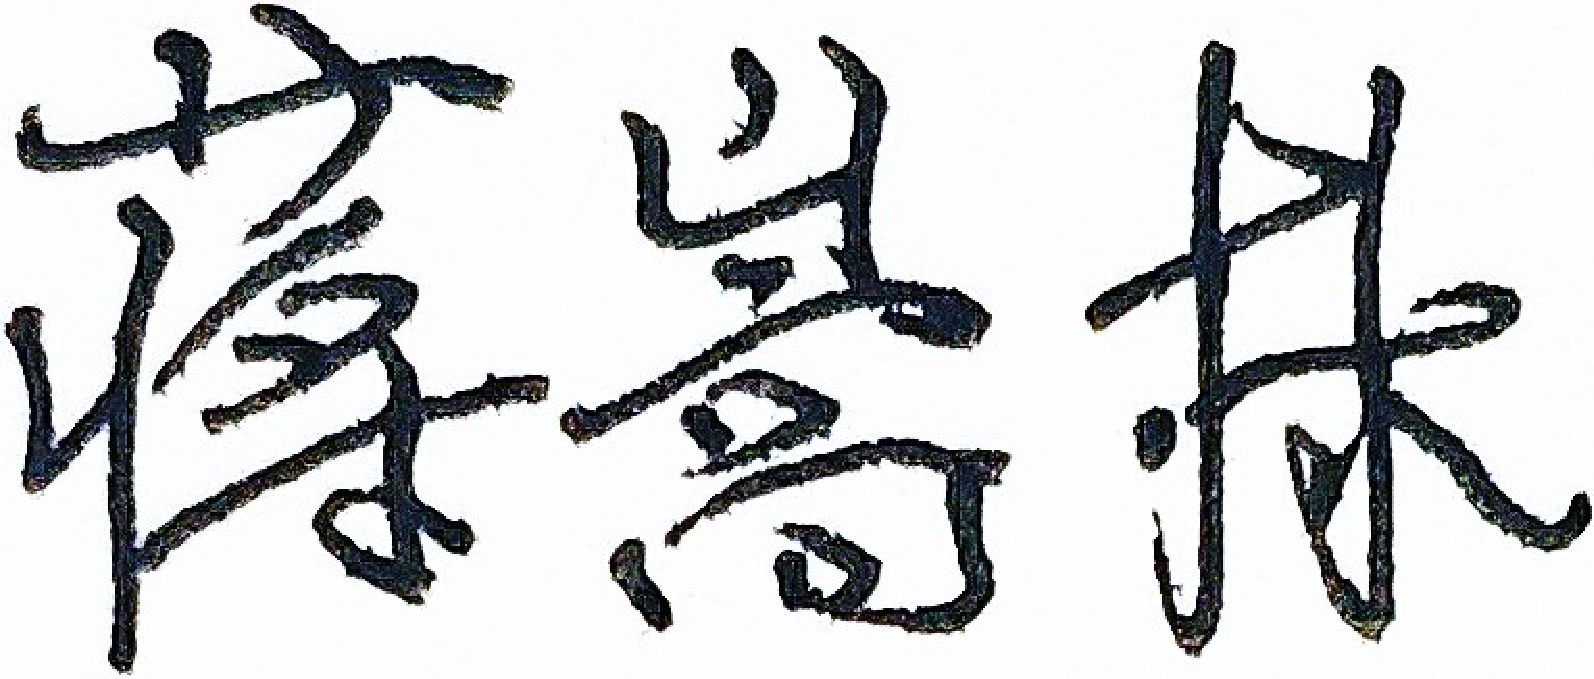
\includegraphics[width=60pt]{author_sig.pdf}
    % }
}
% % 你手写的日期,signature.pdf 改为你的手写的日期文件名
% \mytime{
%     % \raisebox{-5pt}{
%         \includegraphics[width=40pt]{signature.pdf}
%     % }
% }
% % 老师的手写签名,signature.pdf 改为老师的手写签名文件名
% \supervisorsignature{
%     % \raisebox{-5pt}{
%         \includegraphics[width=40pt]{signature.pdf}
%     % }
% }
% % 老师手写的时间,signature.pdf 改为老师的手写的日期文件名
% \teachertime{
%     % \raisebox{-5pSt}{
%         \includegraphics[width=40pt]{signature.pdf}
%     % }
% }
% % 老师手写的成绩
% \recommendedgrade{
%     % \raisebox{-5pt}{
%         \includegraphics[width=40pt]{signature.pdf}
%     % }
% }

\makestatement

%==============================%
% ↑ ↑ ↑ 诚信说明页 授权说明书
%==============================%


%=====%
%论文(设计)成绩:注意2007的模板要求,成绩页在最后,2021要求成绩页在摘要前面
%=====%

% 下面这些注释掉可以去掉成绩、评语什么的
\supervisorcomment{}


\committeecomment{}

\finalgrade{}
% 上面这些注释掉可以去掉成绩、评语什么的

\Grade %这一句才是成绩页,上面是填写


\frontmatter



%中文摘要
\ZhAbstract{
气候变化和环保问题关乎人类未来命运。在石油危机以及全球变暖问题愈发严重的现在,
可再生清洁能源相关研究成为了学界的关注热点。风能,作为触手可得的一种能源,正成为新能
源的主力军之一。准确预测风速,从而保证电网的稳定性,具有十分重大的意义。风速预测
是一个时间序列回归问题,由于风速的波动具有随机性,其影响因素也十分复杂,呈现出
非平稳且非线性的特征,因而对短期风速的预测难度较大。

本文选取数值天气预报中常见的六种气象要素历史数据,包括近地面气温、近地面气压、
近地面空气比湿、地面向下短波辐射、地面向下长波辐射、地面降水率,结合近地面全
风速的历史数据构建短期风速的预测模型。首先,采用当前科研最前沿的自适应噪声完备
集合经验模态分解(CEEMDAN)算法,对上述七种特征历史数据进行分解,将高频噪声和
低频信号进行分离,降低时间序列数据分析的复杂度,从而提高准确性。然后,将分解结
果序列输入由 Facebook 推出的主流时间序列预测框架 Prophet 进行预测以及统计分
析,得到Prophet拟合预测的结果以及统计分析预测得出的趋势分量、累加式季节性分量
、日分量、年分量以及上述分量所对应的预测最大边界和最小边界,进一步降低七种特征
对应时间序列的复杂度,便于神经网络的训练。最终,将所有由 Prophet 分析预测的时
段对应的结果以及分量输入进一个由三层门控循环单元(GRU)构成的深度学习模型,采
用最新科研成果 Nadam 优化器 以及 Huber损失函数训练模型,输出预测的时段对应的
近地面全风速,从而达成预测实际的短期风速的目的。

为了验证模型的实际效果,本文选取了甘肃中电酒泉第四风力发电有限公司附近(北纬
40.65 度,东经 96.95 度)的2017年1月1日0时整至2018年12月31日21时整
\footnote{此处所述时间均为协调世界时(UTC, Universal Time Coordinated)。}间
隔三小时的历史数据,使用均方误差(MSE)、平均绝对误差(MAE)、平均绝对误
差百分比(MAPE)、均方根误差(RMSE)、决定系数($R^2$)等多项指标,以及对模型的预
测结果进行可视化分析,与只使用近地面全风速历史数据、未进行时间序列分解剔除噪声、
只使用单一模型的情况进行对比,对模型全方面综合评估。结果表明,使用本文提出的模型
,预测短期风速的精度会明显提升,因而具有优越性。
}{风速影响因素,短期风速预测,组合模型,自适应噪声完备集合经验模态分解,Prophet,门控循环单元神经网络,深度学习,数据科学}


%英文摘要
\EnAbstract{\fontspec{Times New Roman} {
Climate change and environmental issues matter the destiny of mankind. 
With the oil crisis and global warming becoming more and more serious,
renewable energy related research has become a hot spot which
attracts great attention from academic. Wind, as a readily available 
energy source, is becoming the mainstream in renewable energy. As a result,
it is of great significance to accurately predict the wind speed
so that power system stability can be ensured. Wind speed forecast
is a time series regression problem. Due to the randomness of wind
speed fluctuations, influencing factors for wind speed are very complex,
which shows its characteristics of non-stationary and nonlinear, so it is 
difficult to predict short-term wind speed.

This paper selects the historical data of six common meteorological
elements in numerical weather prediction, including near-surface air 
temperature, near-surface air pressure, near-surface specific humidity,
surface downwelling shortwave radiation, surface downwelling longwave
radiation, and surface precipitation rate. Combine historical time series
data of near-surface total wind speed with the above mentioned elements
and build the short-term wind speed forecasting model. Firstly, CEEMDAN
(Complete Ensemble Empirical Mode Decomposition with Adaptive Noise) 
algorithm, which is at the forefront of current scientific research,
is used to decompose the above seven elements' historical data so that
high-frequency noise and low-frequency signals can be separated, which
eventually leads to reduction of the complexity of time series data
analysis, and improving accuracy. Then, input the decomposed sequence
into Prophet, a mainstream time series forecasting framework developed by
Facebook, for forecasting and statistical analysis, and obtain the
result of Prophet fitting prediction, the trend component, additive
seasonality component, daily component, yearly component as well as
maximum and minimum boundaries of above. These features further help
reduce the complexity of the time series corresponding to the seven
meteorological elements and facilitate the training of the neural
network. Finally, all the predictions and components corresponding
to the time series elements predicted by the Prophet analysis are input
into a deep learning model composed of a three-layer Gated Recurrent Unit
(GRU). Use the latest scientific research results Nadam optimizer and
Huber loss function to train the model, and output the near-surface
total wind speed corresponding to the predicted time period, so that
the actual short-term wind speed can be predicted.

In order to verify the actual effect of the model, this paper selects the
historical data at a location near Gansu Zhongdian Jiuquan Fourth Wind
Power Co., Ltd. (latitude 40.65 degrees north, longitude 96.95 degrees
east) from 0:00 on January 1, 2017 to 21:00 on December 31, 2018 
\footnote{The times mentioned here are all in UTC (Universal Time Coordinated). } 
at three-hour intervals, using various evaluating indicators like
Mean Squared Error (MSE), Mean Absolute Error (MAE), Mean Absolute
Percentage Error (MAPE), Root Mean Squared Error (RMSE), Coefficient of
Determination ($R^2$), etc. The predicted results are visualized, and 
make comparison with the case of only using the near-ground full wind
speed historical data, without time series decomposition to remove
noise, and only using a single model, the model is comprehensively
evaluated in all aspects. The results show that using the model
proposed in this paper, the accuracy of predicting short-term
wind speed will be significantly improved, so it has supremacy.
}}
{wind speed influencing factors; short-term wind speed forecast; 
hybrid model; CEEMDAN; Prophet; GRU; deep learning; data science.
}

%生成目录
\tableofcontents
% \thispagestyle{empty}


%文章主体
\mainmatter

\chapter{绪 \qquad 论}

% !学校要求的规范,绪论是单独的,不是第一章,但是老师们都是让作为第一章,这里我把它放在了论文里,如果你要让在外面,只需要把上面的 \mainmatter 这一句话放在“绪论内容后面,正文第一章前面”即可,也就是 \chapter{latex部分用法简介} 这一句话上面

% \Intro{
\section{选题研究背景及意义}
\subsection{风力发电的前景}
随着工业发展的需要,人类社会对能源的依赖度也在逐步上升。第二次能源革命以来,
传统化石燃料的使用导致了一系列的问题。化石燃料在开采过程中也产生了
一系列的环境问题。以煤炭为例,在开采时,会破坏地表原本的性状,引发滑坡,塌陷
等一系列问题。开采煤炭所产生的废渣也难以处理,产生的污水会对水土环境造成污染。
同时,燃烧化石燃料所产生的二氧化硫($SO_2$)和氮氧化物会形成酸雨、粉尘使空气能
见度降低、一氧化碳(CO)和芳香烃化合物会污染空气。二氧化碳($CO_2$)在大气层中所
占比例的提高,也导致了温室效应与气候变化,从而使得一些极端天气灾害的发生频率
有了显著的升高。然而目前,在世界能源消费占比中,煤炭和石油的比重仍较重要。
我国的能源生产和消费构成中,煤炭在2019年仍在一次能源中占比57.7\%,占据着
主要地位。\cite{能源数据2021王庆一}

当前传统化石燃料,由于其储量的有限性,也正逐步面临枯竭的风险。“绿水青山就
是金山银山”。可再生能源的发展,不仅将会确保绿水青山的存在,而且同时也必然即
将成为金山银山的重要组成部分。过去三十年以来,风能一直保持着最快增长的可再
生能源的记录,是目前全球第二大的可再生能源。风能本质上属于一种气象能源,其
为太阳照射环境下地球表面受热不均,在水平气压梯度力的影响下,由于温差造成大
气对流所产生的一种能量来源。李仲蔚的研究
\cite{李仲蔚2019风力发电企业价值评估研究}估算结果表明,全球可开发
利用的风能资源达到了二百万兆瓦($2\times10^7MW$),是目前全球第一大的可再生
能源水能的10倍。风能因其分布广泛,弥补了水能发电需要的苛刻条件以及对生态自
然环境可能造成不良影响的缺陷。如将预估的可利用风能的1\%加以利用,即可以满
足全球能源的发电使用需求,因而发展潜力极其巨大,十分有望在将来替代水能成为
全球第二大的可再生能源。

\subsection{短期风速预测的意义}
短期风速的主要影响因素分为气象因素和地形因素。其中,气象因素主要包括温度、气压、
湿度等,而地形因素包括地貌、地表障碍等。

对于短期近地面风速的预测能够很好的帮助并促进风能的应用。首先,风力发电厂管理人员
可以通过预测结果优化电力分配,提高发电量;其次,风力发电厂还可以准确的在风速
过大之前对风力发电机指示停机,预防风力发电机的过载损毁,避免或者减少相应的损
失;最后,还可以有效安排好风力发电的电网并网问题,减少因为风速的剧烈波动对电
网电业的稳定性影响,降低运营成本,增加风电场的效益。

对于目前的风速预测研究而言,相关问题主流使用的模型包括传统时间序列模型以及
深度学习模型。他们各自都存在一定的优点和缺陷,单一模型并不能很好的进行预测
\cite{陆冰鉴2020基于}。同时,由于风速数据中往往包含着较大的噪声问题,如何
有效地对其数据集进行降噪处理也是目前研究的方向。由于单一的预测方法无法做到
很好的风速预测,如果能通过组合模型,对其进行精确的预测,将会对风力发电的应
用起到巨大的促进作用。

\section{选题已有研究成果综述}
\subsection{数值预报方法}
数值预报方法使用大气压、气温、相对湿度、风速等数值型数据来作为初始状态,
以流体力学方程和热力学方程为依据来实现整个大气状态模型的构建,通过超级
计算机进行数值计算求解,得到未来天气的预报结果。
\cite{姜兆宇2019多时空尺度的风力发电预测方法综述}

目前数值预报方法已经很成熟,准确性良好,已经广泛地应用到了天气预报中。
但是,由于数值方法需要占用大量的计算资源,难以将时间和空间分辨率
都做得很高,且短期风速中蕴含的噪声较大,因而单纯的数值预报一般不适用于短期风速预报。
朱智慧等人\cite{朱智慧2010T639}基于T639全球中期数值预报产品得到的上海
南汇站24小时风速预报结果利用逐步回归分析、结合Kalman滤波得出的MOS方程
进行订正,结果表明其订正后的精度可以考虑投入实际使用。夏晓玲等人
\cite{夏晓玲2019贵州省数值预报风速产品检验及订正}利用数值预报的
ECWMF,GRAPES和JAPAN模式对于贵州省范围内84个站点的风速预报进行了分析,最终
运用神经网络对3种模式风速预报进行订正,结果表明其误差,正确率订正改善效果
明显,但是相关系数的提高较小。

\subsection{统计与传统机器学习方法}
不同于数值预报方法,统计与传统机器学习方法基于风速历史数据的时间序列,
通过训练机器学习模型来预测未来天气,并且可以对数据进行预处理,从而可以
从历史数据中挖掘出风速数据的潜在规律,因而相对于数值预报方法,模型的训练
和预测更加简单,无需使用超级计算机进行大量的计算。

\begin{itemize}
\item[a. ] 统计方法:
\end{itemize}

经典的统计方法中对于时间序列数据的处理一般采用自回归综合移动平均模型
(ARIMA, AutoRegressive Integrated Moving Average)。其采用过去观
测值的线性函数关系预测未来值。由于风速的时间序列数据普遍是非平稳的,
包含了很强的季节性,因此相关研究普遍采用季节性自回归综合移动平均模
型(SARIMA, Seasonal AutoregRessive Integrated 
Moving Average)SARIMA是Box和Jenkins提出的ARIMA模型的一个扩展,
用于处理具有季节特征的时间序列数据。Sun, R. N.等人\cite{2017Forecast}
基于ARIMA和SARIMA模型提前24小时预测小时平均风速和风力发电量。并进行了
平均相对误差的比较分析。结果表明,SARIMA模型的预测效果明显优于ARIMA模型。

% SARIMA模型一般分为简单季节模型和乘积季节模型:

% \begin{itemize}
% \item[1. ] 简单季节模型:

% 简单季节模型是指序列中的季节效应和其它效应之间是加法关系:
% $$x_t=S_t+T_t+I_t$$

% 简单季节模型通过简单的趋势差分、季节差分之后序列即可转化为平稳,
% 它的模型结构通常如下:
% $$\nabla_D\nabla^dx_t=\frac{\Theta(B)}{\Phi(B)}\varepsilon_t$$

% 其中:
% $$
% \begin{matrix}
% \nabla_Dx_t=\left(1+B^D\right)X_t,{\ }\nabla^dx_t=\left(1-B^D\right)X_t\\
% \Theta(B)=1-\theta_1B-\theta_2B^2-\cdots-\theta_qB^q\\
% \Phi(B)=1-\varphi_1B-\varphi_2B^2-\cdots-\varphi_pB^p\\
% \end{matrix}
% $$

% \item[2. ] 乘积季节模型:

% 由于序列的季节效应、长期趋势效应和随机波动之间有着复杂的相互关联性,
% 简单的季节模型不能充分地提取其中的相关关系。乘积季节模型的构造原理是,
% 短期相关性用低阶 ARMA(p,q) 模型提取,季节相关性用以周期步长s为单位
% 的 ARMA(p,q) 模型提取,假设短期相关和季节效应之间具有乘积关系,
% 模型结构如下:
% $$\nabla^d\nabla_S^Dx_t=\frac{\Theta(B)}{\Phi(B)}\frac{\Theta_S(B)}{\Phi_S(B)}\varepsilon_t$$

% 由于短期相关性和季节效应之间具有乘积关系,所以,可以将差分后的序列拟合成 ARMA(p,q) 模型和 ARMA(p,q) 模型的乘积形式,最终原序列乘积季节模型的完整结构可采取如下表达式:
% $$\Phi(B)\Phi_S(\mathrm{\ }B)\nabla_S^D\nabla^dx_t=\Theta(B)\Theta_S(B)\varepsilon_t$$

% 其中:

% $$
% \begin{matrix}
% \nabla^dx_t=(1-B)^dx_t,\nabla_S^Dx_t=\left(1-B^S\right)^Dx_t\\
% \Phi(B)=1-\varphi_1B-\varphi_2B-\cdots-\varphi_pB^p\\
% \Theta(B)=1-\theta_1B-\theta_2B^2-\cdots-\theta_qB^q\\
% \Phi_S(B)=1-\varphi_1B^S-\cdots-\varphi_PB^{PS}\\
% \Theta_S(B)=1-\theta_1B^S-\cdots-\theta_QB^{QS}\\
% \end{matrix}
% $$

% 该乘积季节模型通常简记为$SARIMA(p,d,q)\times(P,D,Q)_S$。
% \end{itemize}

使用 SARIMA 进行模型构建主要有三个主要步骤,分别为平滑处理、平稳性检验
以及时间序列定阶\cite{Foneone2019时间序列}:

\begin{itemize}
\item 由于SARIMA需要时间序列满足平稳性和非白噪声的要求,所以要首先用差分法
和平滑法(滚动平均和滚动标准差)来实现序列的平稳性操作,并确定确定
季节性与非季节性差分数。
\item 其次利用增强迪基-福勒检验(ADF test, Augmented Dickey Fuller test)判断
序列是否平稳,利用白噪声检验判断序列是否为随机性序列。
\item 最后进行时间序列的定阶。自相关函数 (ACF, AutoCorrelation Function)
和偏自相关函数 (PACF, Partial AutoCorrelation Function) 利用拖尾
和截尾来确定,并应用他们来给时间序列定阶,模型的参数由最大似然 (ML) 
函数估计。
\end{itemize}

SARIMA本身机理决定了SARIMA无法处理非线性
时间序列特征,因而在呈现出非平稳且非线性特征的风速时间序列预测中表现
并不是很好。Haddad等人\cite{haddad2019wind}基于SARIMA方法构建了一个
太阳能和风能预测模型,对于风能预测而言最终效果不是很突出。
Xl, A等人\cite{2021Short}使用SARIMA模型来预测苏格兰沿海地区
的每小时实测风速。结果表明尽管SARIMA在风速预测的性能准确度比方面
相对于循环神经网络方法具有优越性,但是其预测的风速准确度并不是很理想。

\begin{itemize}
\item[b. ] 机器学习方法:
\end{itemize}
 
传统机器学习方法,在风速中应用最广泛的为支持向量回归机(SVR,
Support Vector Regression)。支持向量回归机是支持向量机
(SVM,Support Vector Machine)的一个非常重要的变体,其将SVM
的应用领域从分类变成了回归。SVR的目标是对时间序列输入数据的每个点
通过非线性变换寻找一个最优超平面。不同于SVM的最优超平面需要使得两类
或多类样本点与超平面之间的总偏差最大,SVR的样本点最终只有一类,
并且其最优超平面需要所有的样本点与超平面之间的总偏差最小。

传统的SVR能够对非线性特性的数据有较好的预测能力,然而由于风速呈现
出非平稳的特征,其中所含噪声较多,直接对风速进行预测无法达到很好的
效果。朱霄旬等人\cite{朱霄旬2017遗传算法对}使用一种基于遗传算法
(GA,Genetic Algorithm)的多参数同步优化算法,改进了传统通过相空
间重构法求出SVR预测模型的最优参数的方法,并大大提高了预测精度。
Pan, C.等人\cite{2018Hybrid}首先根据回归率和确定性相结合的联合指数,
对风速序列的可预测性进行了定量分析,然后利用联合指数优化的参数重建风速
序列,通过嵌入维数和延迟时间得到预测模型的最佳输入集。最终利用布谷鸟优化
算法(COA,Cuckoo Optimization Algorithm)优化的SVR模型对风速进行预
测,取得了不错的效果。

\subsection{深度学习方法}

近年来,随着深度学习的发展,深度学习方法在风速预测中的应用越来越广泛。
深度学习由数据驱动,具有十分强大的泛化能力,十分适合处理具有非平稳且
非线性特征的风速时间序列预测。神经网络模型虽然预测效果好,但是
存在训练难度大的问题,对数据集和参数的要求十分高,否则
容易产生过拟合、梯度爆炸、梯度消失等一系列问题。

Shivani等人\cite{Shivani2019A}对传统时间序列统计模型ARIMA和
一个深度学习模型预测风速进行了比较研究。该深度学习模型由长短期记忆网络
(LSTM,Long Short-Term Memory)和循环神经网络
(RNN,Recurrent Neural Network)组合而成,结果凸显了深度学习预测风速
的优越性。Alencar, D. B.等人\cite{alencar2018hybrid}提出了一种基于
SARIMA和反向传播(BP,Back Propagation)神经网络的组合模型方法,
用于多步超前风速预测。并进行了仿真分析。其结果表明,对于不同的预测时段,
该组合模型预测方法的预测精度优于大部分传统算法。朱丽娜的研究
\cite{朱丽娜2021风电}得出结论:LSTM适用于预测非平稳序列风速,Elman神经
网络,一种动态递归神经网络,次之。

\subsection{降噪方法}
由于风速数据的非平稳性,其时间序列数据中往往参杂着较大的噪声。这些噪声
如果不加以平滑处理从而去除,将会严重影响到模型对风速时间序列的预测精度
和泛化能力,加大对其非线性关系的学习难度。常见的信号分解技术基于傅里叶
变换,将时间序列信号从时域变换到频域,从而将高频噪声剔除。这些
信号分解技术包括小波分解(WD,Wavelet Decomposition)、变分模式分解
(Variational Mode Decomposition)、Hilbert-Huang变换
(HHT,Hilbert-Huang Transform)以及经验模式分解
(EMD,Empirical Mode Decomposition)以及基于上述四类方法演化出的
一系列分支。

谢义超\cite{谢义超2021基于}提出了一种基于CEEMDAN分解和改进的LSTM模型。
该模型基于粒子群优化算法(PSO,Particle Swarm Optimization)与样本熵
选择CEEMDAN以及LSTM的超参数,从而让参数达到最优值。最终得出的结果表明,
CEEMDAN分解技术可以极大地提高基于循环神经网络模型的泛化能力,降低模型
的训练难度。王秀的研究\cite{王秀2021基于}基于小波变换,通过SARIMA和
LSTM模型的组合,提升了对短期风速的预测精度。

\section{论文研究内容与组织结构}

随着数据科学的发展,使用开箱即用(Out of the box)的数据分析框架
已经成为数据科学研究的一种新潮流。在这之中包括了流行的机器学习框架
scikit-learn,以及时间序列数据处理预测框架Prophet。

由于注意到直接使用Prophet框架来进行非平稳非线性的风速预测效果并不佳,因而
本文基于上述前人研究成果,决定选用CEEMDAN分解技术,并使用当前最新循环神经
网络结构GRU,结合Prophet框架,形成CEEMDAN-Prophet-GRU模型。同时结合数值
预报方法提供的灵感,将其他天气要素特征也输入到模型中,提高模型的泛化能力,
最终验证模型的优越性。论文的结构如下:

第一章:绪论。主要讲述选题缘由,风速问题研究背景以及意义,以及对现有研究
方法的综述。

第二章:数据来源及特征提取。主要讲述特征的选取原因以及数据集的制作过程,并
对选取数据集的性状进行了分析。

第三章:使用技术介绍。主要讲述CEEMDAN分解技术、Prophet、GRU网络、
Nadam 优化器 以及 Huber损失函数的原理介绍。

第四章:模型的建立和评估。主要讲述模型的训练以及调参过程、评估指标介绍
与分别用单一模型的情况进行对比。

第五章:总结与展望。对全文进行总结,指出创新点与有待进一步改进研究的方向。

% }


% % =======正文从第一章开始
% \setcounter{chapter}{0}

\chapter{数据来源及特征选取}
\section{数据来源}
本文数据来源于中国区域地面气象要素驱动数据集(1979-2018)
\cite{8028b944-daaa-4511-8769-965612652c49},该数据集常用于数值天气
预报。该数据集包括近地面气温、近地面气压、近地面空气比湿、近地面全风速、
地面向下短波辐射、地面向下长波辐射、地面降水率共7个气象要素。数据时间
分辨率为3小时,水平空间分辨率为0.1°,为NETCDF格式。
\cite{37cab0ac-d066-4fb9-aa9c-1cf50d601096}

该数据集基于世界上现有的GLDAS数据、普林斯顿再分析数据、GEWEX-SRB辐射
数据和TRMM降水数据,并整合了中国气象局的常规气象观测数据。原始数据来
自卫星遥感数据、再分析数据与气象局的观测数据,并去除了非物理范围值,
对于缺失数据采用ANUSPLIN统计插值。该数据集的精度介于气象局的观测数据
和卫星遥感数据之间,优于世界上现有的再分析数据。\cite{6bab74c1-f2dd-4e24-a833-81f33bedf9b1}

\section{特征选取与数据集的制作}
本文数据集基于上述中国区域地面气象要素驱动数据集(1979-2018)构建而成,
通过Python语言选取了甘肃中电酒泉第四风力发电有限公司附近(北纬
40.65 度,东经 96.95 度)的2017年1月1日0时整至2018年12月31日21时整
\footnote{此处所述时间均为协调世界时(UTC, Universal Time Coordinated)。}
共5840条数据。数据格式为CSV(逗号分隔值,Comma-Separated Values)文件,包
含数据内容如下:

\begin{table}[H]
    \centering
    \caption{选取特征说明}
    \begin{tabular}{cccccc}
    \toprule
    特征 & 名称 & 单位 & 含义 \\
    \midrule
    ds & 日期 & UTC & 数据格式为:YYYY-MM-DD HH:MM:SS \\
    lrad & 地面向下长波辐射 & $W/m^2$ & 从当前时间1.5小时前开始的3小时平均值 \\
    prec & 地面降水率 & $mm/h$ & 从当前时间3小时前开始的3小时平均值 \\
    pres & 近地面气压 & $Pa$ & 近地面(距地面2米处)瞬时值 \\
    shum & 近地面空气比湿 & 比值,无单位 & 近地面(距地面2米处)瞬时值 \\
    srad & 地面向下短波辐射 & $W/m^2$ & 从当前时间1.5小时前开始的3小时平均值 \\
    temp & 近地面气温 & $K$ & 近地面(距地面2米处)瞬时值 \\
    wind & 近地面全风速 & $m/s$ & 近地面(距地面2米处)瞬时值 \\
    \bottomrule
    \end{tabular}
    \label{features}
\end{table}

\section{特征数据分析}


\chapter{使用技术介绍}
\section{CEEMDAN分解}

\section{Prophet}

\section{GRU}

\section{Nadam优化器}

\section{Huber损失函数}


\chapter{模型的建立和评估}
\section{模型评价指标介绍}

\section{七种特征数据的CEEMDAN分解}

\section{仅使用风速历史时间序列数据的Prophet模型}

\section{仅使用风速历史时间序列数据的Prophet-GRU模型}

\section{多特征CEEDMAN-Prophet-GRU模型}

\section{上述三种模型的对比评估}


\chapter{总结与展望}

%论文后部
\backmatter


%=======%
%引入参考文献文件
%=======%
\bibdatabase{bib/database}%bib文件名称 仅修改bib/ 后部分
\printbib
% \nocite{*} %显示数据库中有的,但是正文没有引用的文献


\Appendix


这里是附录页,附上你的程序或必要的相关知识

{\bfseries 编译方式:} XeLaTeX -->BibTeX --> XeLaTeX-->XeLaTeX



\Thanks

时光荏苒,岁月如梭。转眼间,近四年的本科生活就要结束了。这四年是充满了挑战
和挫折的四年,同时也是充满了丰收和果实的四年。值此毕业论文致谢之际,
我首先需要特别感谢的是我的毕业论文指导老师,兰州大学信息科学与工程学院的任超
副教授。任老师治学严谨,对我的论文写作极其认真负责。每当我遇到困难请教任老师
时,任老师总能事无巨细地耐心讲解。同时,任老师极高的专业素养与渊博的学识也十分
令我钦佩!在任老师带领的论文写作过程中,我的科研素养得到了极大地提高,获得了许多
十分宝贵的知识和经验。

其次,我要感谢兰州大学提供的一流教学环境与教育资源,兰州大学信息科学与工程
学院的各位老师的专业教导,以及兰州大学信息科学与工程学院2018级计算机科学与技术
基础理论班的各位同学,以及舍友和其他同学的支持与鼓励。四年的朝夕相处,是他们
让我拓宽了视野,掌握了基本的计算机专业知识和技能,并且让我获得了学习的动力,
为我的继续深造以及未来工作打好了坚实的基础,从而让我能够更好地为社会贡献自己
的力量。在后续的学习工作生活中,我必将以梦为马,不负韶华!

最后,我要感谢大学四年父母对我的默默关爱和支持,让我能够顺利地完成本科学业。
父母对我的无私且伟大的爱,是我在黑暗中的灯塔,给予了我不断前行的动力。

另外,本文使用的数据集下载于“国家青藏高原科学数据中心”(http://data.tpdc.ac.cn)。
在写作时从GitHub中获取并使用了兰州大学2016级物理科学与技术学院本科生余航
制作的“兰州大学本科生2021学士学位毕业论文LaTeX模板”,在此也一并致谢。

\end{document}